\documentclass{beamer}
\usetheme{Madrid}
\usecolortheme{beaver}
\title{Mass \& Balance}
\subtitle{Lesson 1}
\author{Alberto Botto Poala}
\institute{AeC Biella}
\date{\today}

\begin{document}

\begin{frame}
\titlepage
\end{frame} 

\begin{frame}
\frametitle{Table of Contents}
\tableofcontents
\end{frame} 

\section{Massa vs Quantità di Moto vs Forza Peso}
\begin{frame}
\frametitle{massa, quantità di moto e forza}
\textbf{massa} $(kg)$: è una grandezza scalare propria dei corpi materiali che ne determina il comportamento dinamico quando sono soggetti all'influenza di forze esterne.
\begin{figure}
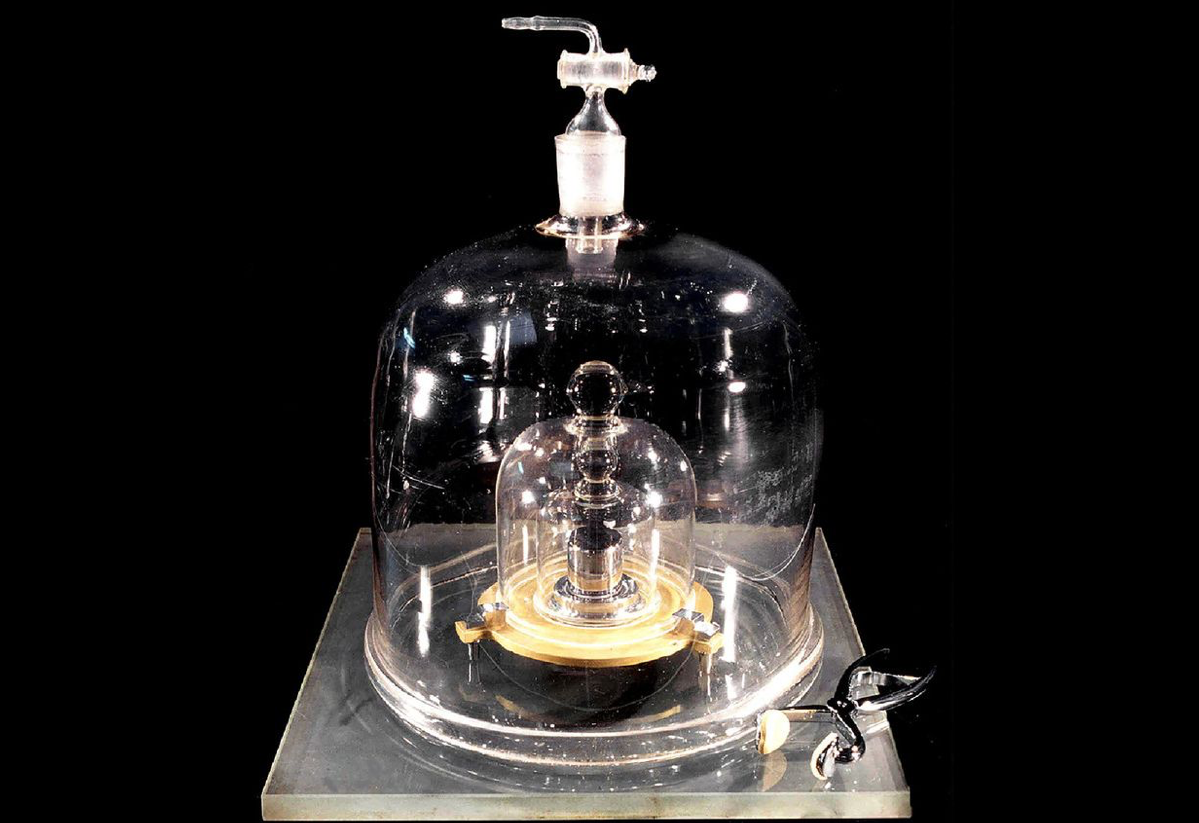
\includegraphics[scale=0.14]{./images/1kg}
\end{figure}
\pause

\textbf{quantità di moto} $(kg \ m/s)$: è una grandezza vettoriale definita come il prodotto della massa dell'oggetto per la sua velocità.
$$\vec{p} = m \vec{v}$$
\pause

\textbf{forza} $(N = kg \ m / s^2 )$: Seconda Legge di Newton 
$$\vec{F} = m \  \vec{a}$$ 
\end{frame}

\begin{frame}
\frametitle{forza e accelerazione di gravità}
\textbf{forza di gravità}: La forza di gravità (forza peso, o più semplicemente peso) è, in fisica classica, la forza che un campo gravitazionale (ad esempio quello terrestre) esercita su un corpo avente massa.
\pause

$$\vec{F}_{grav} = m \  \vec{g}, \ \ dove \  \vec{g} = 9.81 \ m/s^2$$ 
\pause

\begin{figure}
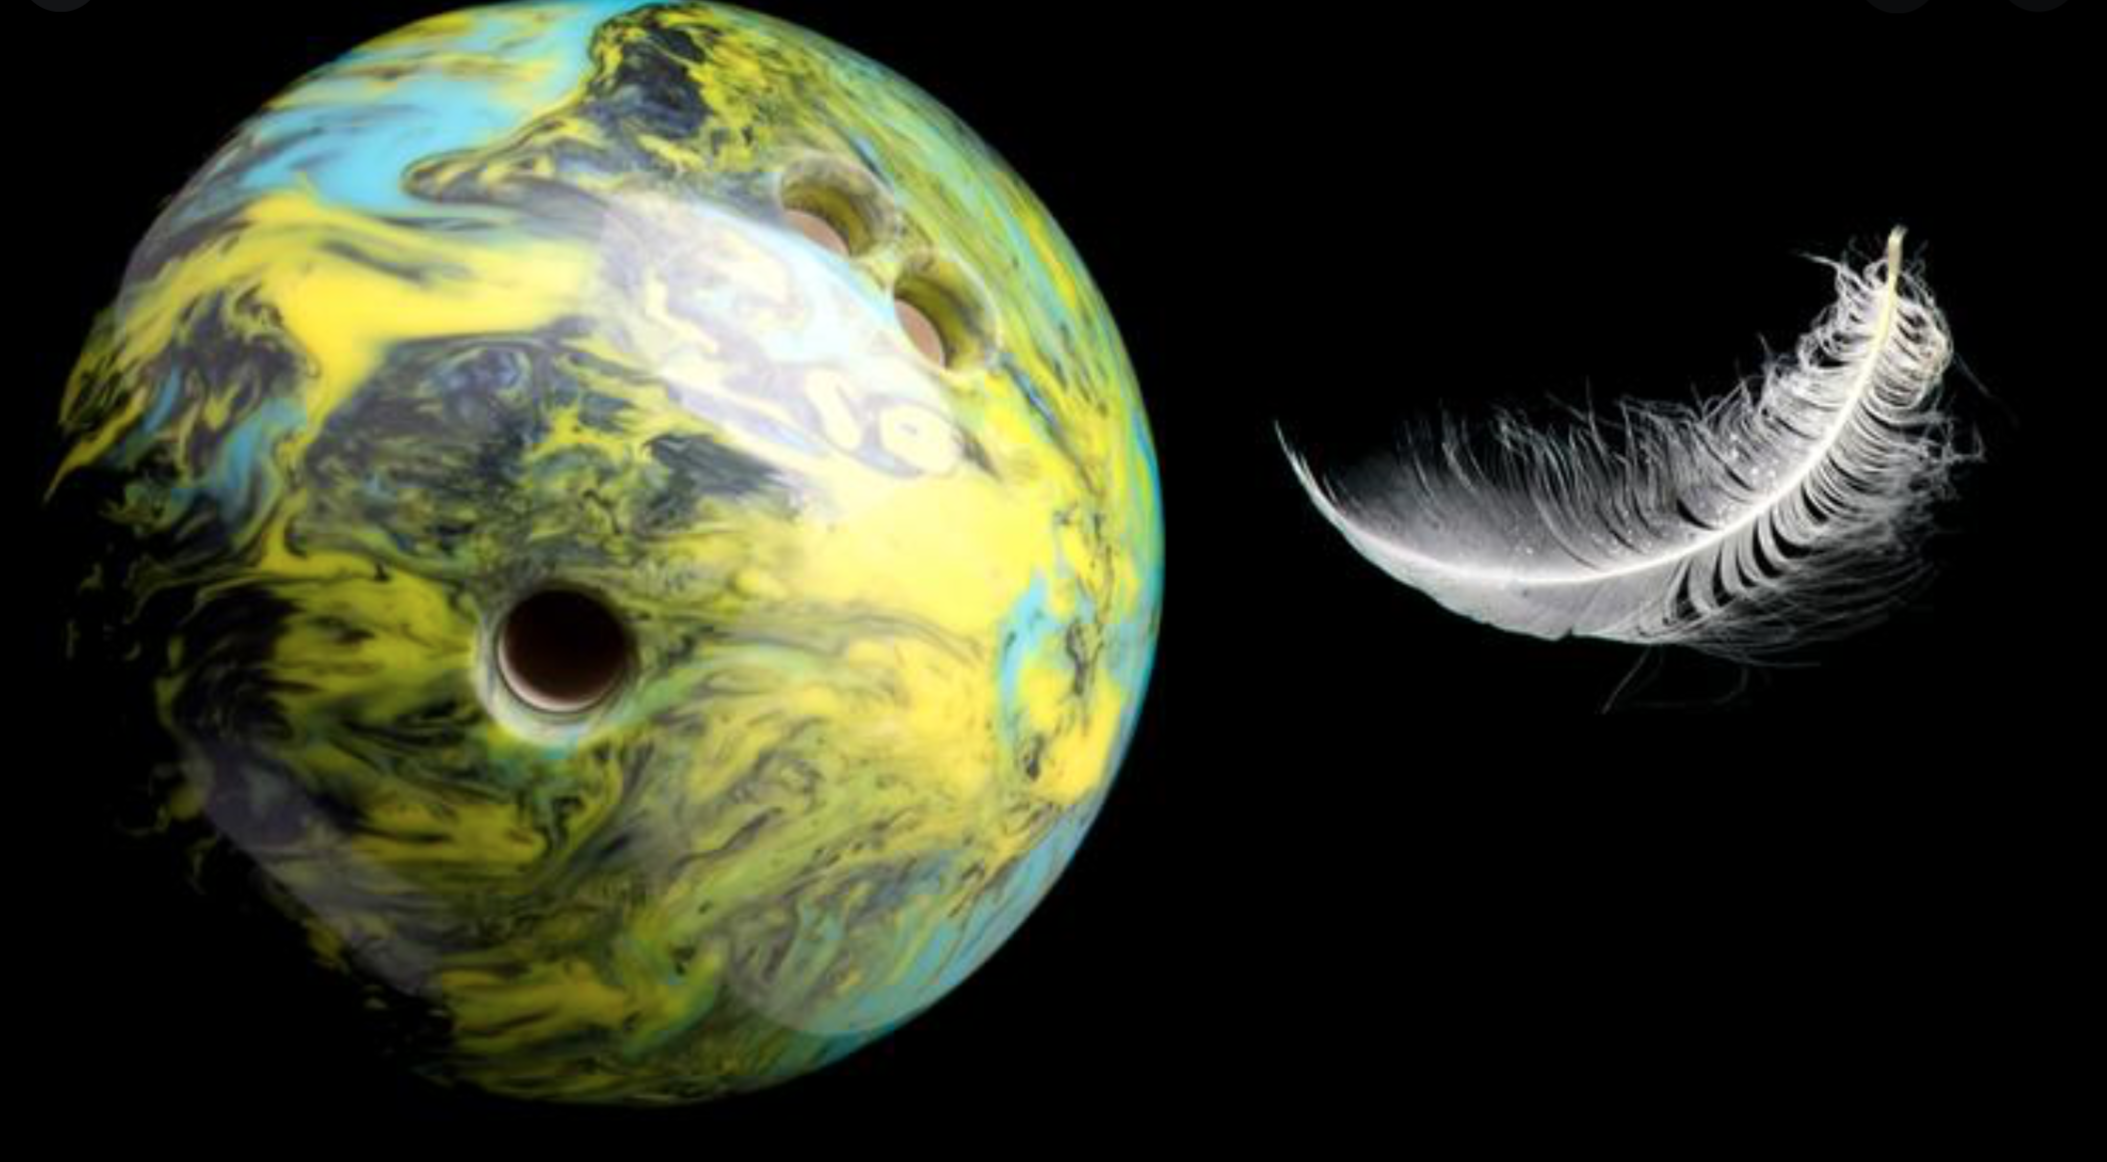
\includegraphics[scale=0.25]{./images/feather}
\end{figure}

\end{frame}

\begin{frame}
\frametitle{centro di massa}
\textbf{centro di massa}: in meccanica classica, il centro di massa (o centro di gravità, CG, o baricentro) di un sistema è il punto geometrico corrispondente al valor medio della distribuzione della massa del sistema nello spazio.
\pause

\begin{figure}
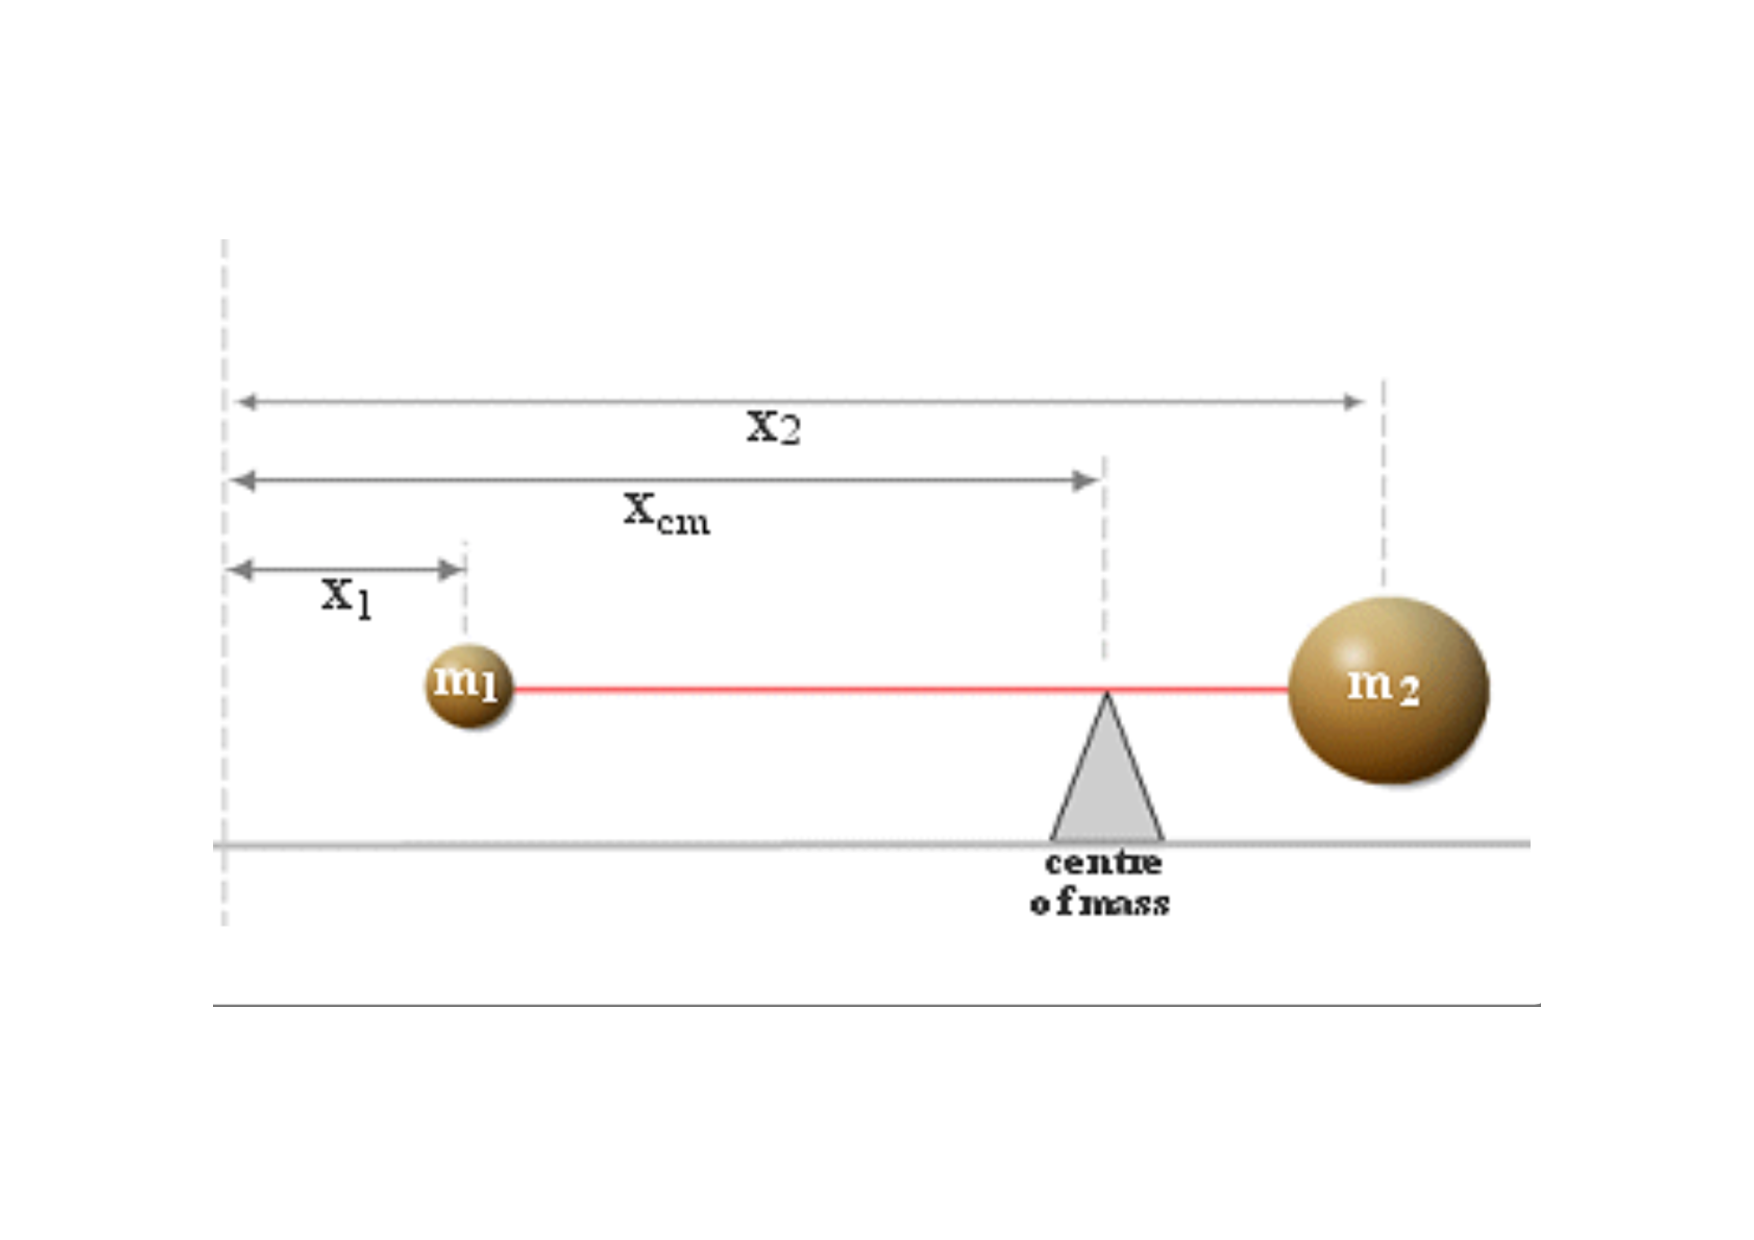
\includegraphics[scale=0.2]{./images/cdm}
\end{figure}
\pause

$$x_{cm} (m_1 + m_2) = x_1 m_1 + x_2  m_2$$ \\
%\pause

%$$x_{cm}  = \frac{x_1 m_1 + x_2  m_2}{(m_1 + m_2)}$$
\end{frame}

\begin{frame}
\frametitle{centro di massa}
\begin{figure}
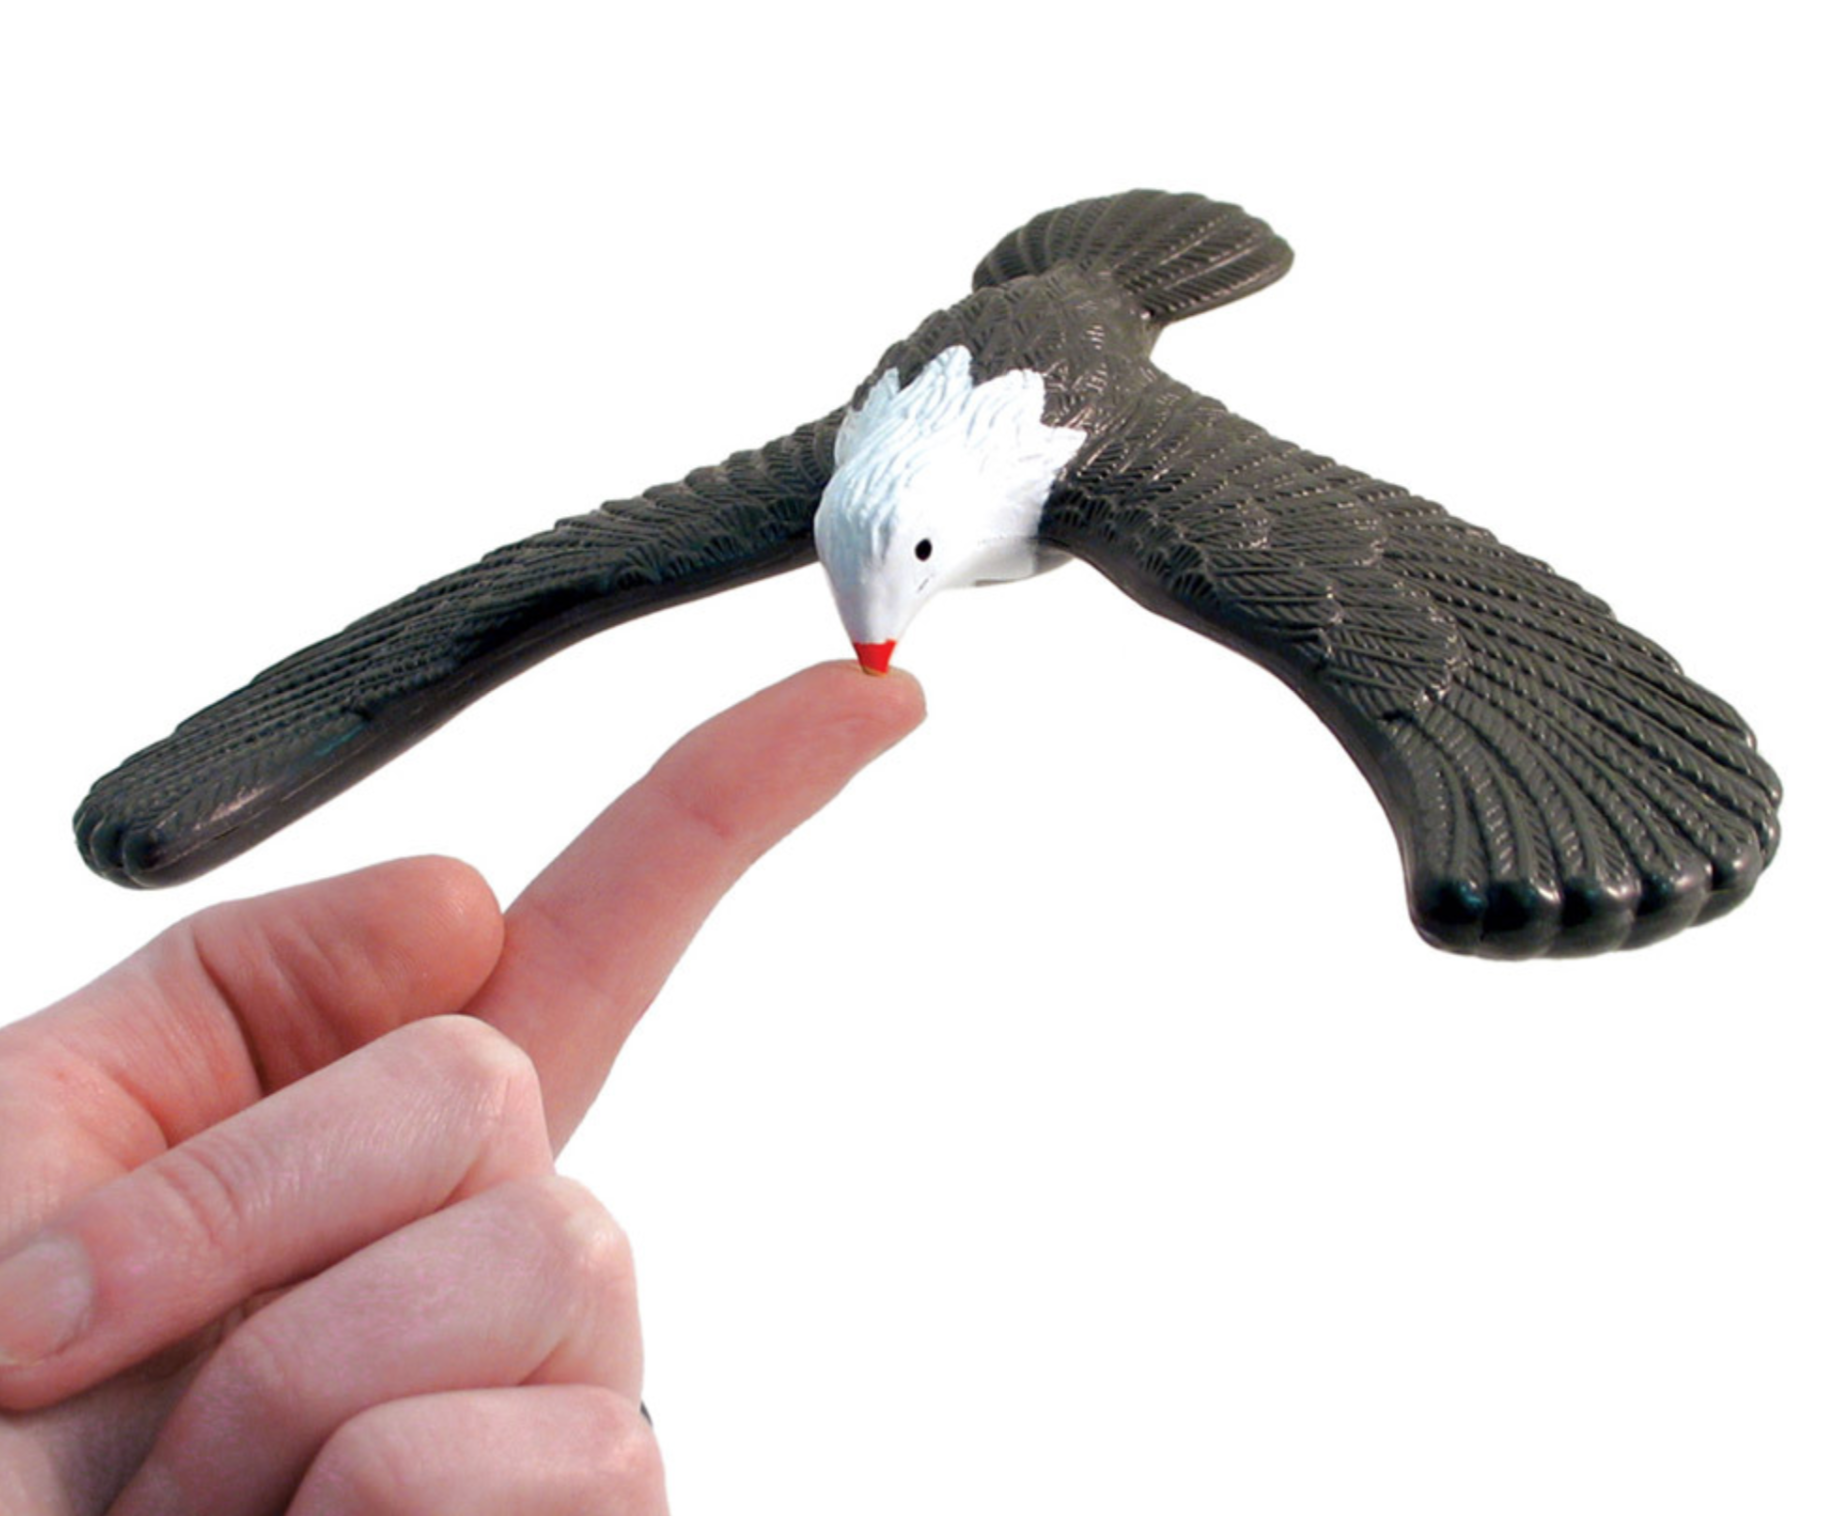
\includegraphics[scale=0.25]{./images/bird}
\end{figure}
\end{frame}

\begin{frame}
\frametitle{esperimento nel mondo reale}
\begin{figure}
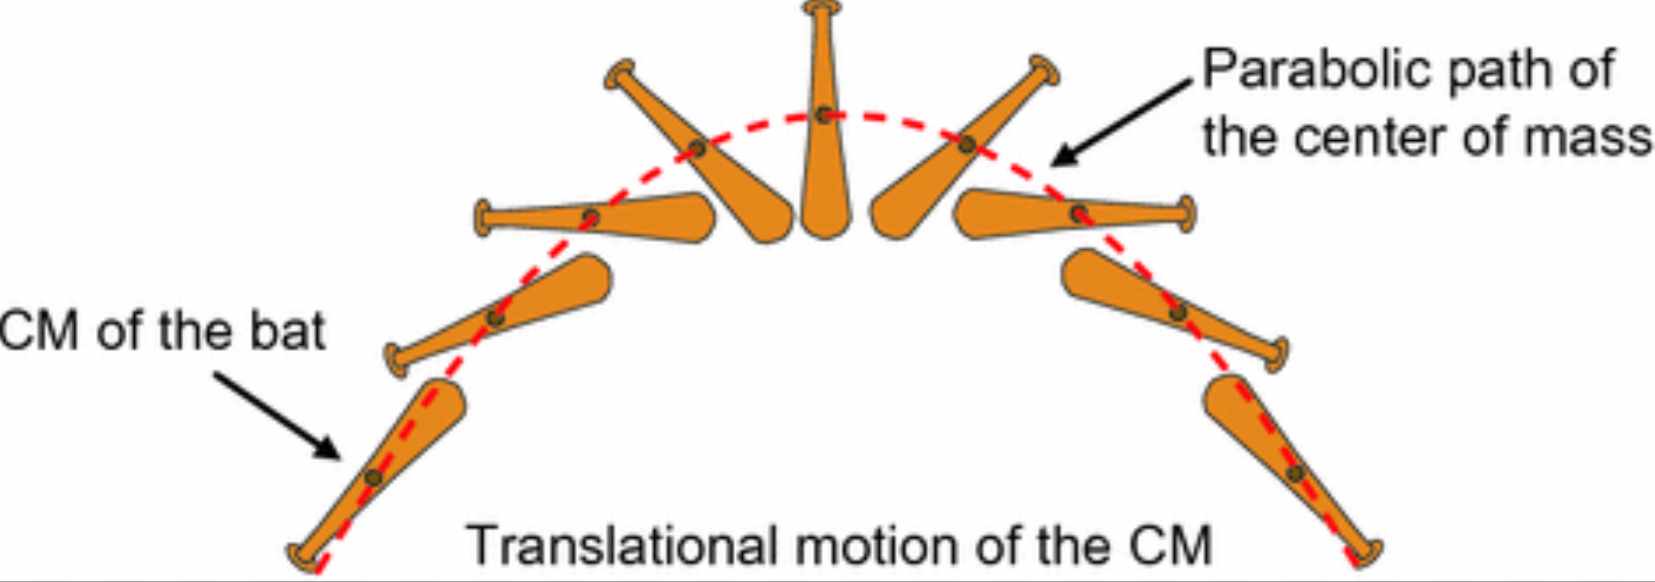
\includegraphics[scale=0.33]{./images/bat}
\caption{risultato dell'imprimere una forza su un oggetto lontano dal centro di massa}
\end{figure}
\end{frame}

\section{Momento d'Inerzia vs Momento Angolare vs Momento}
\begin{frame}
\frametitle{traslazioni e rotazioni}
\centering
\begin{tabular}{|c|c|} \hline
        traslazioni & rotazioni  \\ \hline
          massa & momento d'inerzia \\ 
        $m$ &  $I = m r^2$   \\ \hline
        quantità di moto & momento angolare \\
            $\vec{p}$ &  $\vec{L} = \vec{r} \times \vec{p}$   \\ \hline
            forza & momento \\
            $\vec{F}$ &  $\vec{M} = \vec{r} \times \vec{F}$  \\ \hline
      \end{tabular}
\end{frame}

\begin{frame}
\frametitle{cos'è il momento angolare?}
\begin{figure}
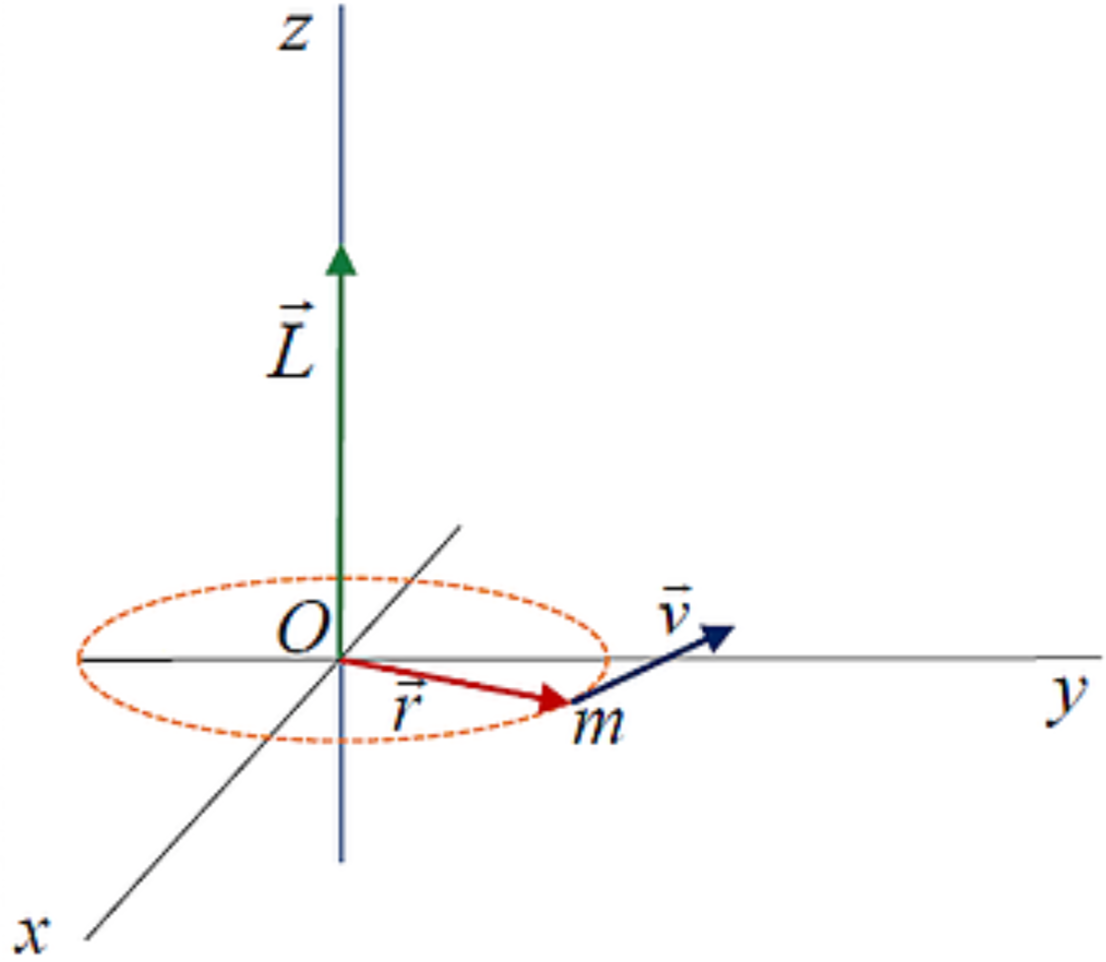
\includegraphics[scale=0.33]{./images/momentoangolare}
\caption{il momento angolare $\vec{L}$ è la controparte della quantità di moto $\vec{P}$ nelle rotazioni}
\end{figure}
\end{frame}

\begin{frame}
\frametitle{esempio di conservazione di $\vec{L}$}
\begin{figure}
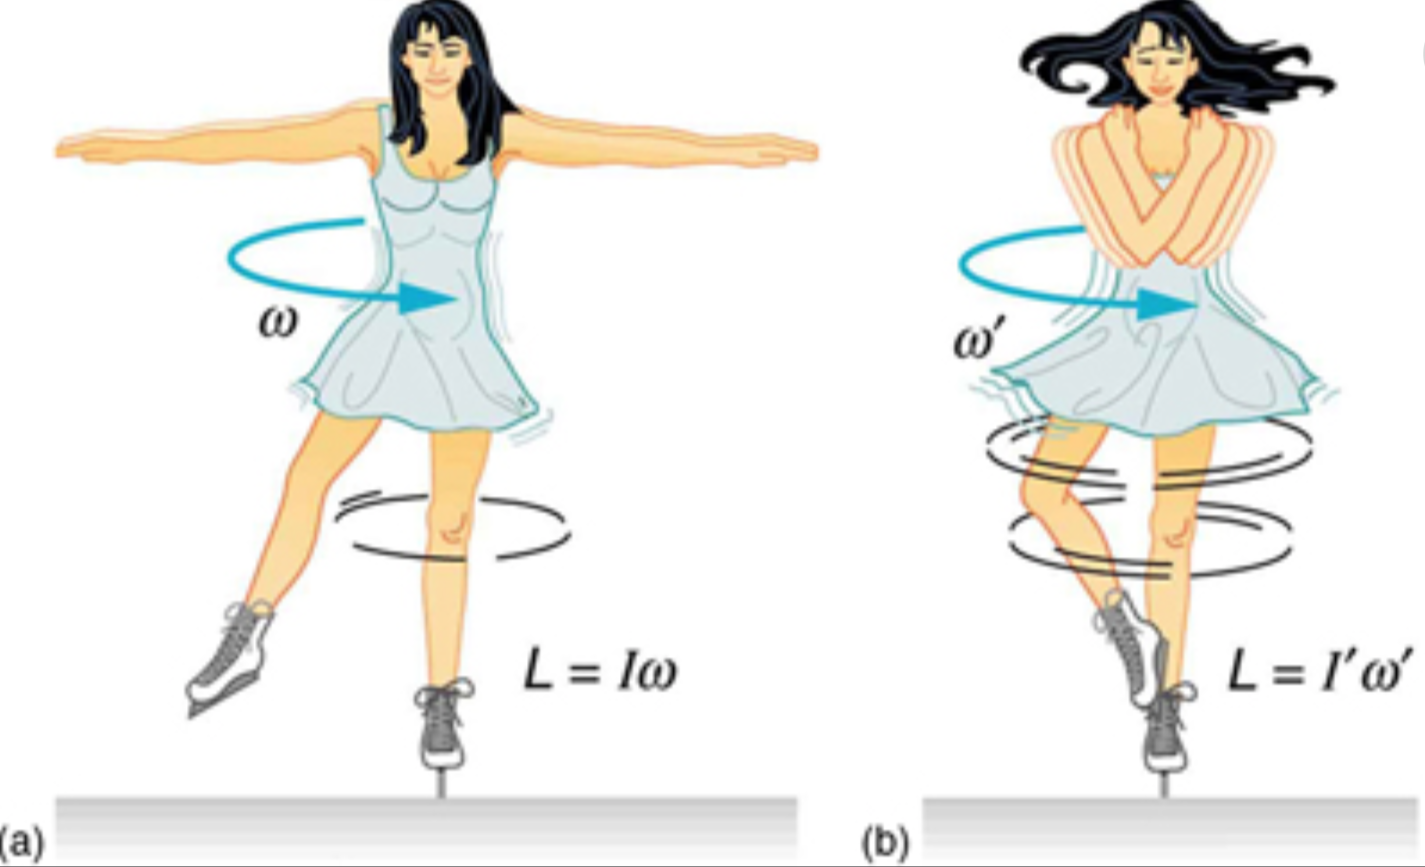
\includegraphics[scale=0.33]{./images/dancer}
\caption{il momento angolare $\vec{L}$ è una quantità conservata}
\end{figure}
\end{frame}

\begin{frame}
\frametitle{Momenti su un aereo di linea}
\begin{figure}
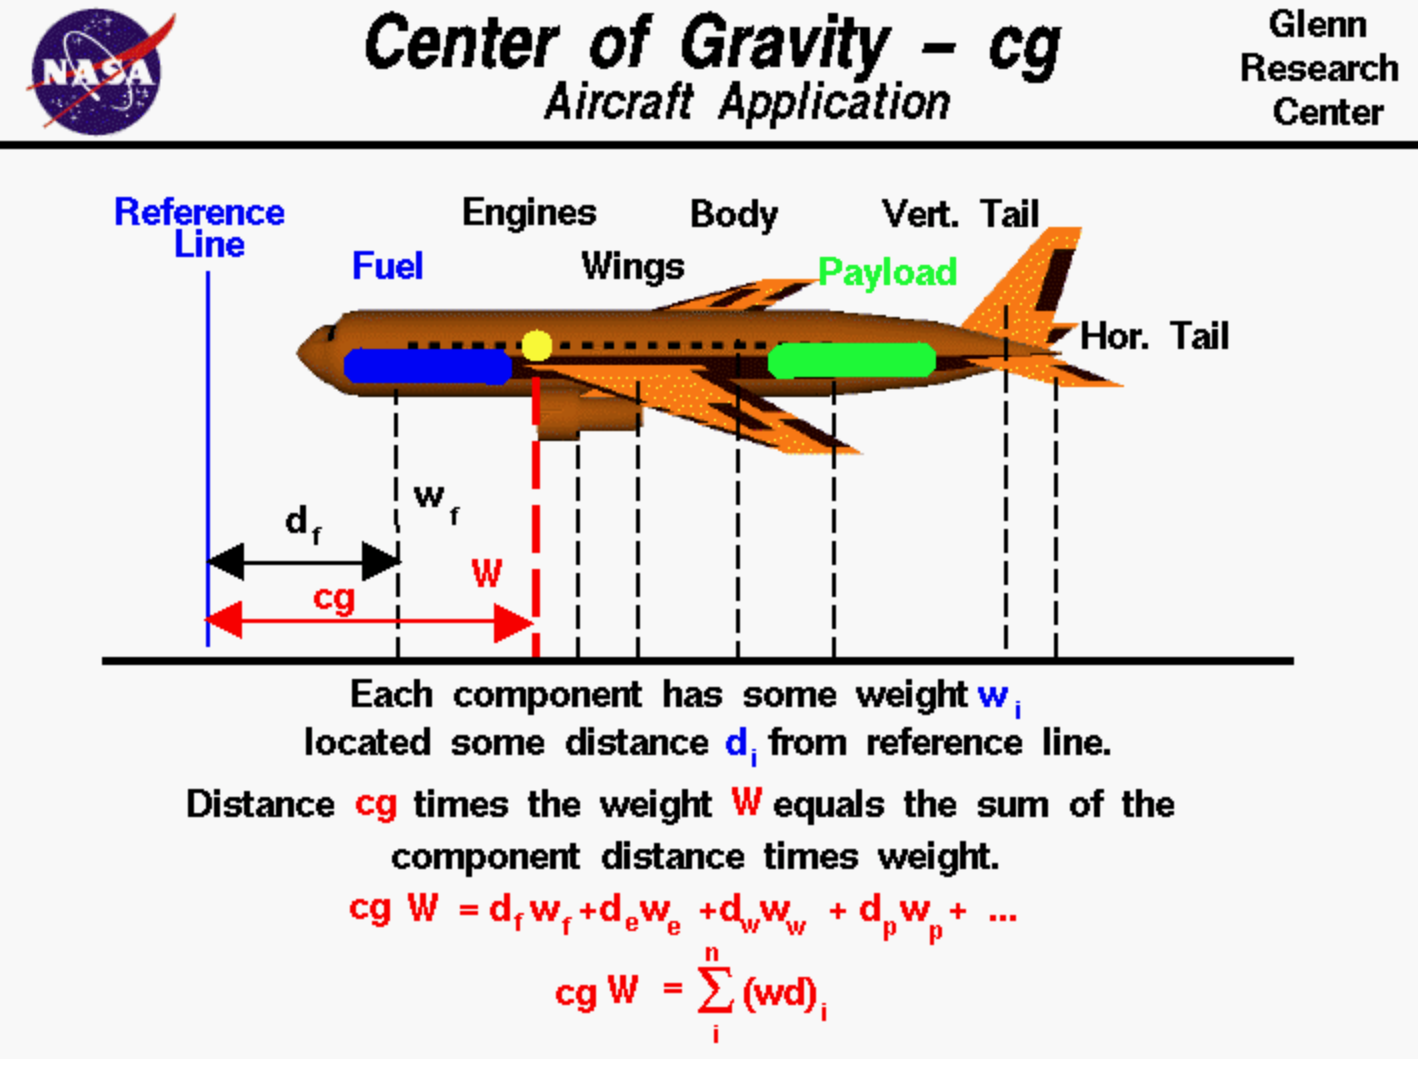
\includegraphics[scale=0.33]{./images/complexmab}
\caption{un aereo di linea è sottoposto a molteplici momenti che devolo bilanciarsi. \textit{Credit: Glenn Research Center}}
\end{figure}
\end{frame}

\end{document}
